
\begin{figure}
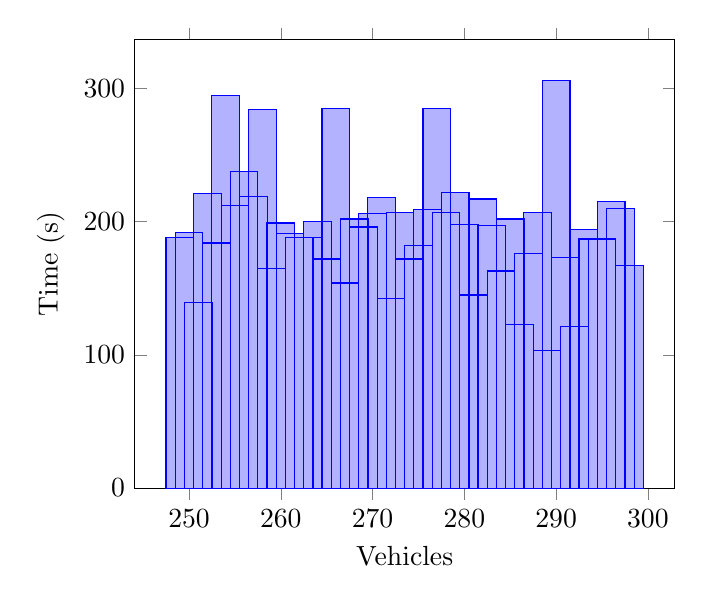
\begin{tikzpicture}
\begin{axis}[
legend style={anchor=west},
xlabel=Vehicles,
ylabel=Time (s),
ymin=0,
ybar,
]
\addplot coordinates {
(298, 167)
(296, 215)
(297, 210)
(295, 187)
(292, 121)
(293, 194)
(290, 306)
(291, 173)
(270, 206)
(271, 218)
(272, 142)
(274, 172)
(275, 182)
(276, 209)
(277, 285)
(278, 207)
(279, 222)
(249, 188)
(294, 187)
(273, 207)
(258, 284)
(259, 165)
(252, 221)
(250, 192)
(251, 139)
(256, 238)
(257, 219)
(254, 295)
(255, 212)
(280, 198)
(289, 103)
(288, 207)
(281, 145)
(283, 197)
(282, 217)
(285, 202)
(284, 163)
(287, 176)
(286, 123)
(263, 188)
(262, 188)
(261, 191)
(260, 199)
(267, 154)
(266, 285)
(265, 172)
(264, 200)
(269, 196)
(268, 202)
(253, 184)
};

\end{axis}
\end{tikzpicture}
\label{tik:time:0:91}
\caption{0 percent diving with GSC on route $91$}
\end{figure}
